\chapter{Przerzutnik D wyzwalany poziomem}

\section{Budowa układu}

\begin{itemize}
    \item Należało zbadać przerzutnik D wyzwalany poziomem korzystając z układu 7475 (\ref{link:7475})
        \begin{figure}[H]
            \centering
            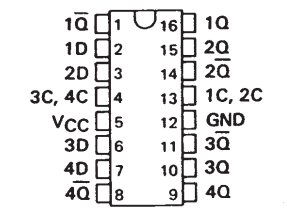
\includegraphics[width=0.5\textwidth]{img/schemes/7475_pins.png}
            \caption{Piny TTL 7475}
            \label{D_poziom:piny}
        \end{figure}
    \item Korzystając z jednego z impulsatorów (górnego) podajemy wartości na wejście D przerzutnika.
    \item Drugi z impulsatorów (dolny) służy jako zegar.
    \item Wyjście przerzutnika \textbf{Q} oraz $\overline{\textbf{Q}}$ (piny 16, 1) zostały wyprowadzone do diod elektroluminescencyjnych znajdujących się na prawej stronie płytki.
        \begin{figure}[H]
            \centering
            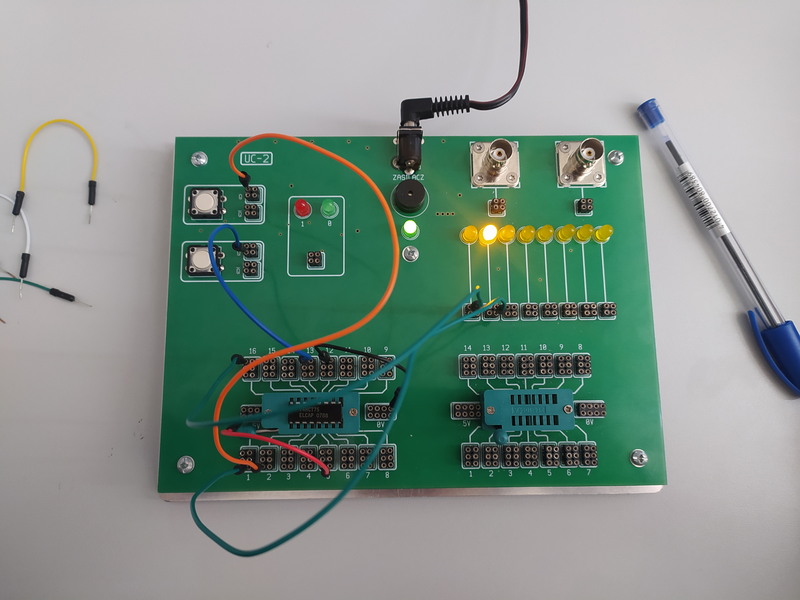
\includegraphics[width=0.7\textwidth]{img/5_4/1653500525041_scaled.png}
            \caption{Zbudowany przerzutnik D}
            \label{D_poziom:zbudowany}
        \end{figure}
        
        \begin{figure}[H]
            \centering
            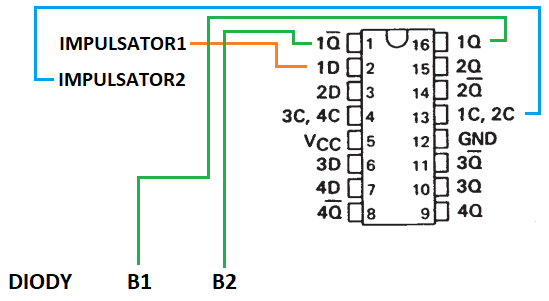
\includegraphics[width=\textwidth]{img/schemes_w_pins/5_4_w_pins.png}
            \caption{Schemat z połączonymi pinami}
            \label{D_poziom:schemat_z_pinami}
        \end{figure}
\end{itemize}

\section{Testowanie układu}

\begin{itemize}
    \item Przetestowano układ dla różnych wejść D (górny impulsator) oraz C (dolny impulsator).
    \item Dla wartości \textbf{C=0}:
       \begin{figure}[H]
            \centering
            \begin{subfigure}[H]{0.48\textwidth}
                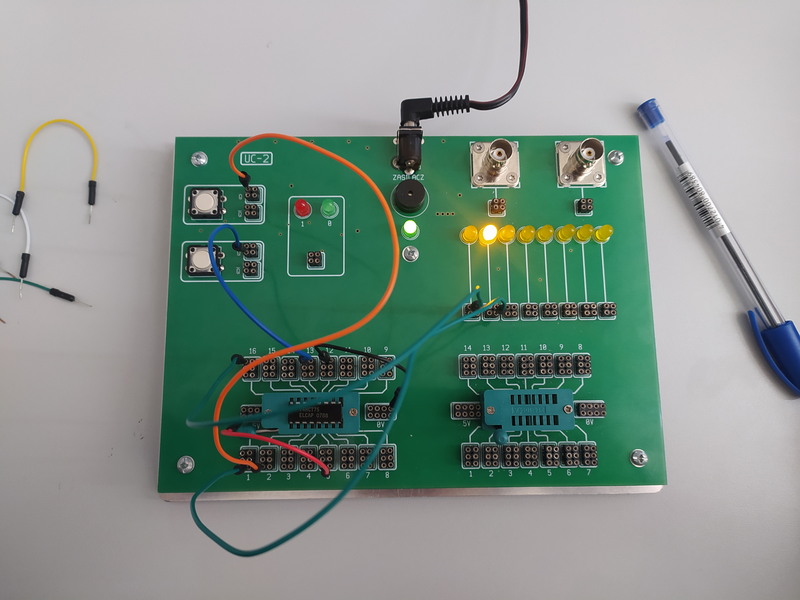
\includegraphics[width=\textwidth]{img/5_4/1653500525041_scaled.png}
                \caption*{\textbf{D=0}, \textbf{C=0}, \textbf{Q=0}, $\overline{\textbf{Q}}$\textbf{=1}}
            \end{subfigure}
            \begin{subfigure}[H]{0.48\textwidth}
                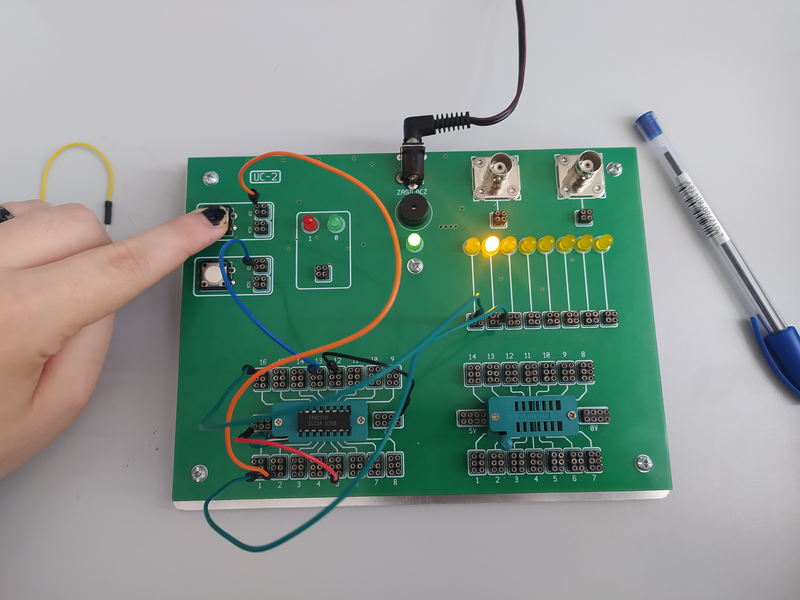
\includegraphics[width=\textwidth]{img/5_4/1653500525025_scaled.png}
                \caption*{\textbf{D=1}, \textbf{C=0}, \textbf{Q=0}, $\overline{\textbf{Q}}$\textbf{=1}}
            \end{subfigure}
        \end{figure}
        
\pagebreak
        
    \item Dla wartości \textbf{C=1}:
        \begin{figure}[H]
            \centering
            \begin{subfigure}[H]{0.48\textwidth}
                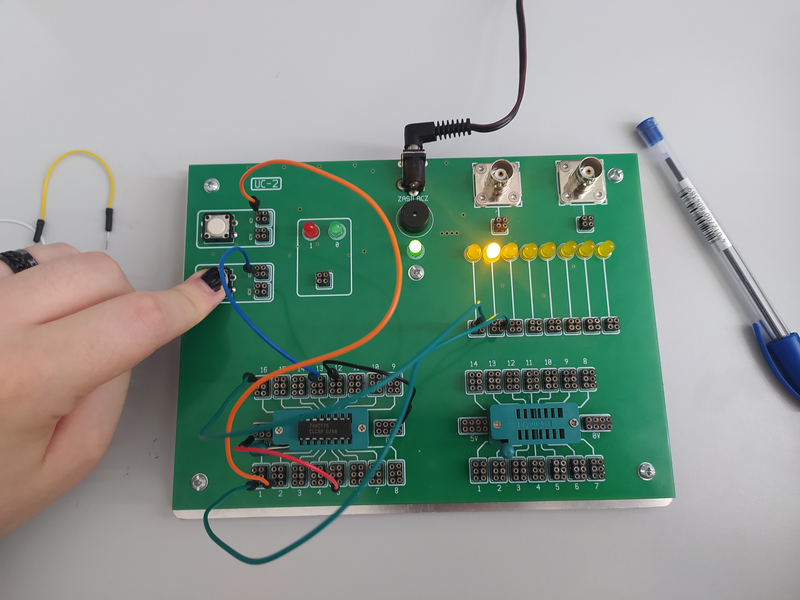
\includegraphics[width=\textwidth]{img/5_4/1653500524989_scaled.png}
                \caption*{\textbf{D=0}, \textbf{C=1}, \textbf{Q=0}, $\overline{\textbf{Q}}$\textbf{=1}}
            \end{subfigure}
            \begin{subfigure}[H]{0.48\textwidth}
                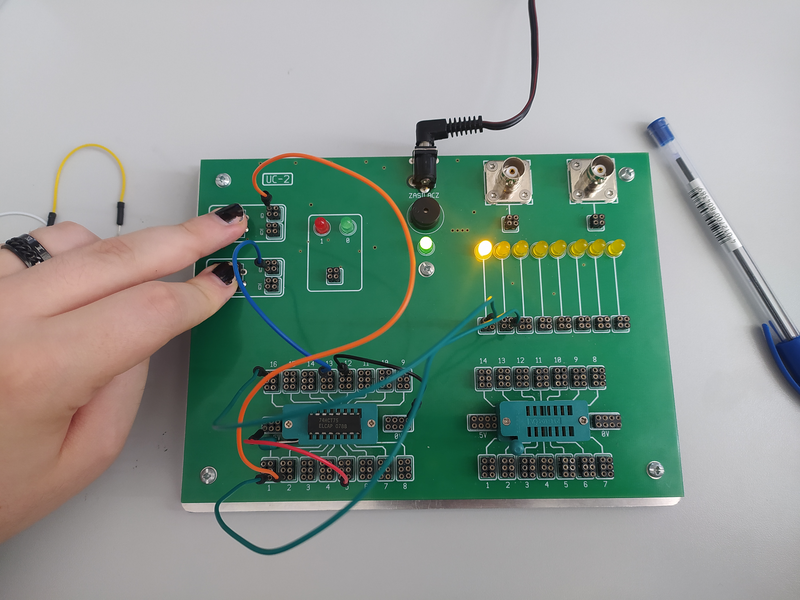
\includegraphics[width=\textwidth]{img/5_4/1653500524969_scaled.png}
                \caption*{\textbf{D=1}, \textbf{C=1}, \textbf{Q=0}, $\overline{\textbf{Q}}$\textbf{=1}}
            \end{subfigure}
        \end{figure}
    \item Testowanie ``\textbf{zatrzasku}``. Początkowo ustawiono wyjście Q=1 za pomocą D=1, C=1. Następnie ustawiono C=0 tak aby aktualny stan przerzutnika został zachowany.
        \begin{figure}[H]
            \centering
            \begin{subfigure}[H]{0.48\textwidth}
                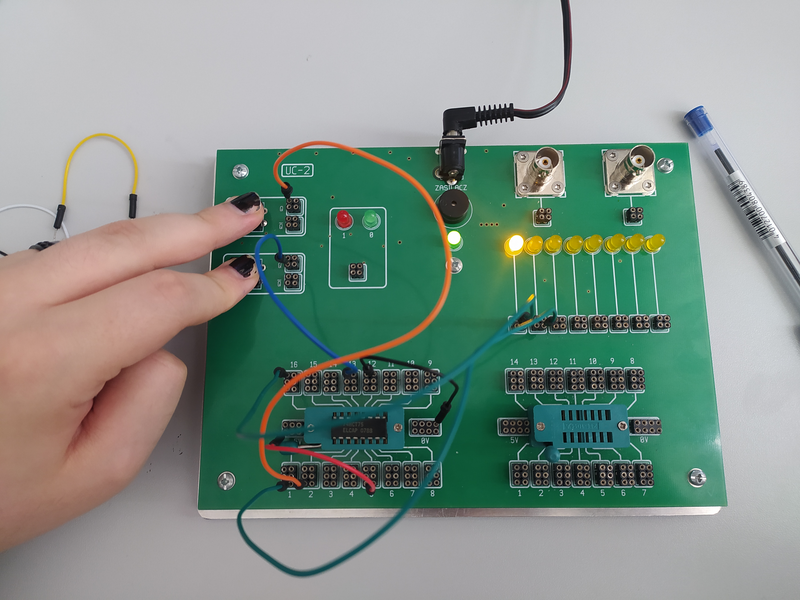
\includegraphics[width=\textwidth]{img/5_4/1653500524945_scaled.png}
                \caption*{\textbf{D=1}, \textbf{C=1}, \textbf{Q=1}, $\overline{\textbf{Q}}$\textbf{=0}}
            \end{subfigure}
            \begin{subfigure}[H]{0.48\textwidth}
                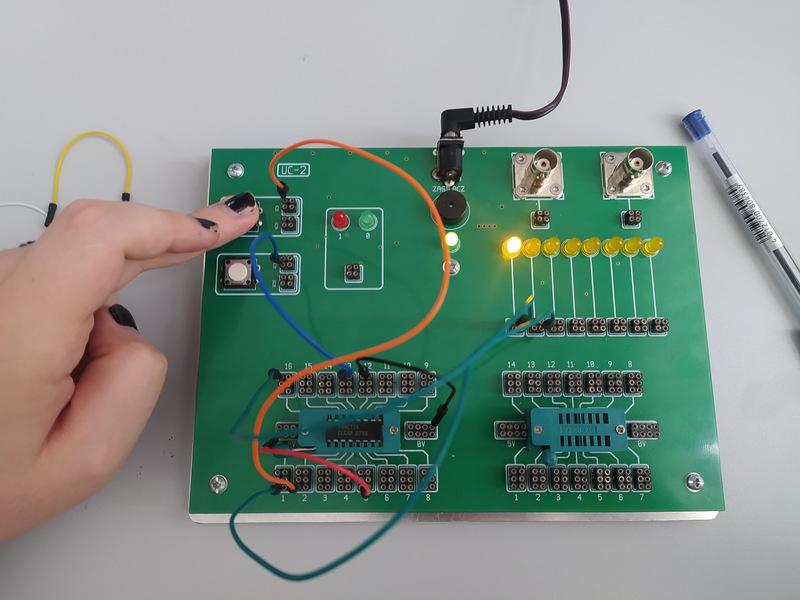
\includegraphics[width=\textwidth]{img/5_4/1653500524916_scaled.png}
                \caption*{\textbf{D=1}, \textbf{C=0}, \textbf{Q=1}, $\overline{\textbf{Q}}$\textbf{=0}}
            \end{subfigure}
            \begin{subfigure}[H]{0.48\textwidth}
                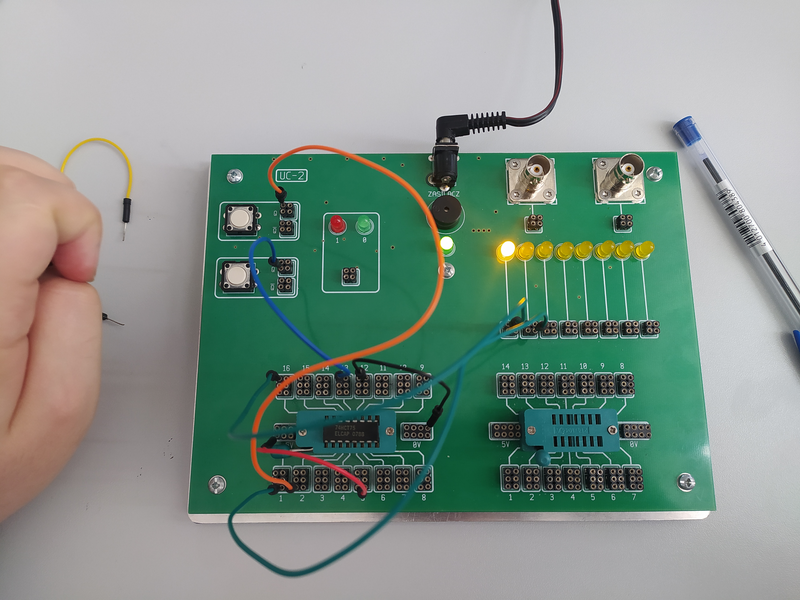
\includegraphics[width=\textwidth]{img/5_4/1653500524895_scaled.png}
                \caption*{\textbf{D=0}, \textbf{C=0}, \textbf{Q=1}, $\overline{\textbf{Q}}$\textbf{=0}}
            \end{subfigure}
        \end{figure}
    \item Uzyskana doświadczalnie tabela prawd zgadza się z teoretyczną (\ref{przerzutnik_D:tabela_stanow}). Układ działał \textbf{poprawnie}. 
\end{itemize}